\documentclass[12pt, titlepage]{article}

\usepackage{xcolor} % for different colour comments
\usepackage{tabto}
\usepackage{mdframed}
\mdfsetup{nobreak=true}
\usepackage{xkeyval}
\usepackage{tabularx}
\usepackage{float}
\usepackage{booktabs}
\usepackage{hyperref}
\hypersetup{
    colorlinks,
    citecolor=black,
    filecolor=black,
    linkcolor=red,
    urlcolor=blue
}
\usepackage[skip=2pt, labelfont=bf]{caption}
\usepackage{titlesec}
\usepackage{graphicx}
\graphicspath{ {images/} }
\usepackage{enumitem}

%% the following adds another section level by redefining the paragraph
%% source:  http://tex.stackexchange.com/questions/60209/how-to-add-an-extra-level-of-sections-with-headings-below-subsubsection
\setcounter{secnumdepth}{4}

\titleformat{\paragraph}
{\normalfont\normalsize\bfseries}{\theparagraph}{1em}{}
\titlespacing*{\paragraph}
{0pt}{3.25ex plus 1ex minus .2ex}{1.5ex plus .2ex}


%% Comments
\newif\ifcomments\commentstrue

\ifcomments
\newcommand{\authornote}[3]{\textcolor{#1}{[#3 ---#2]}}
\newcommand{\todo}[1]{\textcolor{red}{[TODO: #1]}}
\else
\newcommand{\authornote}[3]{}
\newcommand{\todo}[1]{}
\fi

\newcommand{\wss}[1]{\authornote{magenta}{SS}{#1}}
\newcommand{\ds}[1]{\authornote{blue}{DS}{#1}}


\newcommand*\justify{%
  \fontdimen2\font=0.4em% interword space
  \fontdimen3\font=0.2em% interword stretch
  \fontdimen4\font=0.1em% interword shrink
  \fontdimen7\font=0.1em% extra space
  \hyphenchar\font=`\-% allowing hyphenation
}

\newcommand{\getCurrentSectionNumber}{%
  \ifnum\c@section=0 %
  \thechapter
  \else
  \ifnum\c@subsection=0 %
  \thesection
  \else
  \ifnum\c@subsubsection=0 %
  \thesubsection
  \else
  \thesubsubsection
  \fi
  \fi
  \fi
}



\makeatother



\begin{document}
\title{\bf Platform Perils\\[\baselineskip]\Large User Guide}
\author{Steven Palmer\\$\langle$palmes4$\rangle$\\Chao Ye\\$\langle$yec6$\rangle$}
\date{\today}
	
\maketitle

\pagenumbering{roman}
\tableofcontents
\listoftables
\listoffigures


\begin{table}[b]
\caption*{\bf Revision History}
\begin{tabularx}{\textwidth}{p{3.5cm}p{2cm}X}
\toprule {\bf Date} & {\bf Version} & {\bf Notes}\\
\midrule
February 28, 2016 & 1.0 & Created document\\
February 29, 2016 & 1.1 & Finished draft\\
\bottomrule
\end{tabularx}
\end{table}

\newpage

\pagenumbering{arabic}

\section{Introduction}
The purpose of this guide is to provide installation instructions as well as an overview of the game.  The guide is structured as follows:

\begin{itemize}
  \item The first part of the guide deals with system requirements and offers step-by-step installation instructions (see \hyperref[sec:gettingstarted]{\S\ref*{sec:gettingstarted}}).
  \item The second part of the guide serves as an instruction manual for the game (see \hyperref[sec:basics]{\S\ref*{sec:basics}}, \hyperref[sec:edit]{\S\ref*{sec:edit}})
  \item The final part of the guide provides additional help in the form of FAQ and troubleshooting sections (see \hyperref[sec:faq]{\S\ref*{sec:faq}}, \hyperref[sec:trouble]{\S\ref*{sec:trouble}})
\end{itemize}

\subsection{Definitions}
The definitions used throughout this guide are listed in \hyperref[tab:terminology]{Table~\ref*{tab:terminology}}.


\begin{table}[H]
\caption{List of Terms} \label{tab:terminology}
\renewcommand{\arraystretch}{1.2}
\begin{tabularx}{\textwidth}{p{4cm}X}
\toprule {\bf Term} & {\bf Definition}\\
\midrule
\texttt{installer} & Refers to the \texttt{gamebuilder.tar.gz} archive that contains an automated installer and the files required to build the game.  When extracted, a folder structure with a root directory called \texttt{gamebuilder/} is created.\\
\texttt{game directory} & The game directory can be found at \texttt{\justify gamebuilder/game/} (see \texttt{installer}) \\
\texttt{source directory} & The source directory can be found at \texttt{\justify gamebuilder/source/} (see \texttt{installer}) \\
\texttt{build directory} & The build directory can be found at \texttt{\justify gamebuilder/source/build/} (see \texttt{installer}) \\
\bottomrule
\end{tabularx}
\end{table}
\section{Getting Started}
\label{sec:gettingstarted}
\subsection{System Requirements}
\subsubsection{Hardware Requirements}
Running the game requires a system with a GPU that supports OpenGL v3.3 or higher.\footnote{Consult the specifications of your GPU to determine the highest supported version of OpenGL.}  Hardware requirements related to performance have not been assessed.
\subsubsection{Software Requirements}

Platform Perils is compatible with the following operating systems:
\begin{itemize}
  \item \texttt{Windows 7}
  \item \texttt{Mac OS X 10.6 and higher}
  \item \texttt{Linux (confirmed working on the Arch Linux distribution)}
\end{itemize}

\noindent The following software will be required to install the game:
\begin{itemize}
  \item \texttt{CMake}
  \item \texttt{gcc}
  \item \texttt{make}
\end{itemize}

\noindent Please refer to the installation instructions in the following section for further details.

\subsection{Installation Instructions}
A cross-platform compatible installer is included with the game.  To use the installer you will need to download and install the latest release of \href{https://cmake.org/}{CMake}.  Make sure that \texttt{\bf CMake} can be run from the terminal/command prompt (you may need to edit your PATH variable).



\subsubsection{Installing on Windows}
\begin{enumerate}
  \item Download and install \href{http://sourceforge.net/projects/mingw-w64/}{mingw-w64}, which will be used to compile the game and the required libraries.  Install with default settings (threads should be set to POSIX) and ensure that \texttt{\bf gcc.exe}, \texttt{\bf g++.exe}, and \texttt{\bf mingw32-make.exe} can be run from the command prompt (you may need to edit your PATH variable).\footnote{\texttt{\bf mingw-w64} is a fork of \texttt{\bf mingw} and much more up to date.  Regular \texttt{\bf mingw} installations do not include libraries that are required to build the game and its required libraries.  If you have a previous installation of \texttt{\bf mingw} you can either replace it or keep both versions.}

  \item Open a command prompt and navigate to the pre-made \texttt{build} directory (\texttt{\justify gamebuilder/source/build/}).
  \item Run the command\\\\
   ${}$\qquad \texttt{cmake -G "MinGW Makefiles" ..}\\\\
    to invoke cmake.  A makefile (as well as many other files) will be generated in the \texttt{build} directory.

  \item Run the command\\\\
   ${}$\qquad \texttt{mingw32-make}\\\\
    to begin building the libraries and the game.  This will build all of the necessary libraries as well as the game.  The build process should take 1 to 2 minutes.

  \item Run the command\\\\
  ${}$\qquad \texttt{mingw32-make install}\\\\
  to install the game to the \texttt{game} directory.  All of the files required to run the game will be moved to this directory.

\end{enumerate}

\subsubsection{Installing on Mac OS X and Linux}


\begin{enumerate}
  \item Open a terminal and navigate to the pre-made \texttt{build} directory\\ (\texttt{\justify gamebuilder/source/build/}).
  \item Run the command\\\\
   ${}$\qquad \texttt{cmake -G "Unix Makefiles" ..}\\\\
    to invoke cmake.  A makefile (as well as many other files) will be generated in the \texttt{build} directory.

  \item Run the command\\\\
   ${}$\qquad \texttt{make}\\\\
    to begin building the libraries and the game.  This will build all of the necessary libraries as well as the game.  The build process should take 1 to 2 minutes.

  \item Run the command\\\\
  ${}$\qquad \texttt{make install}\\\\
  to install the game to the \texttt{game} directory.  All of the files required to run the game will be moved to this directory.
\end{enumerate}

\subsubsection{Other Operating Systems}
The game must be installed manually on other operating systems.  To perform a manual installation you will need to download and compile the following libraries:

\begin{enumerate}
  \item \href{https://chipmunk-physics.net/}{Chipmunk2D}
  \item \href{http://www.glfw.org/}{GLFW}
  \item \href{http://www.glew.org/}{GLEW}
  \item \href{http://kcat.strangesoft.net/openal.html}{OpenAL Soft}
  \item \href{https://github.com/vancegroup/freealut}{FreeALUT}
\end{enumerate}

\noindent The game can then be built using the source files and headers located in the \texttt{src} and \texttt{include} folders in the \texttt{source} directory.  Be sure to merge all of the include folders that come with the libraries with the \texttt{include} folder found in the \texttt{source} directory folder.  All of the aforementioned libraries must be linked when compiling the game (as well as any operating system dependent libraries you may require).

\subsection{Running the Game}
Once the game is installed, it can be run via the executable found in the \texttt{game} directory.  When running the game for the first time, use of the terminal/command prompt is recommended in case any error messages arise.  If an error is encountered, refer to \hyperref[sec:trouble]{\S\ref*{sec:trouble}} for troubleshooting.


\section{Game Basics}
\label{sec:basics}
Platform Perils focuses on a nameless hero who finds himself lost in a world full of dangerous hazards.  It is up to you to help the hero navigate safely through a series of perilous stages so that he can return home.


\subsection{Stages}
\noindent Each stage in the game begins with the hero situated at a designated start position.  If the hero is killed by a hazard in the stage, he will restart at the start position.  The goal of each stage is to reach the arch (see \hyperref[fig:arch]{Figure~\ref*{fig:arch}}) in the fastest time possible while avoiding the deadly hazards. When a stage is completed for the first time, the next stage is unlocked and becomes playable.  Stages become progressively more difficult.

\begin{figure}[H]
\begin{center}
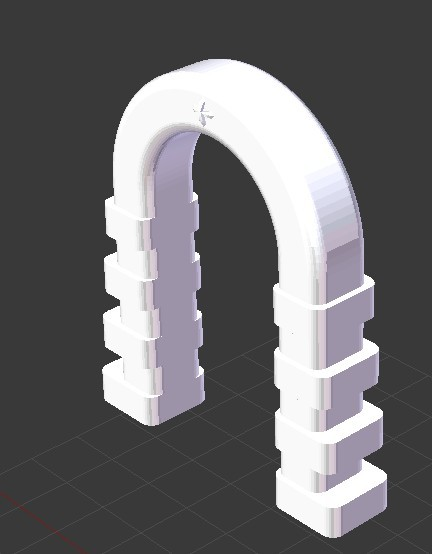
\includegraphics[width=0.25\textwidth]{door}
\caption{End of stage arch.} \label{fig:arch}
\end{center}
\end{figure}

\subsubsection{Hazards}
The hazards that will be encountered in the game stages are summarized in \hyperref[tab:hazards]{Table~\ref*{tab:hazards}}.  The visual representation of each hazard is given in \hyperref[fig:hazards]{Figure~\ref*{fig:hazards}}

\begin{table}[H]
\caption{Hazards} \label{tab:hazards}
\renewcommand{\arraystretch}{1.2}
\begin{tabularx}{\textwidth}{p{4cm}X}
\toprule {\bf Hazard} & {\bf Description}\\
\midrule
Boulder & The boulder is a dangerous hazard that will crush any person in its path.  When the boulder has stopped rolling is no longer hazardous and may even be used as a platform.\\
Spikes & Spikes are a fatal hazard that are frequently found on the tops and bottoms of platforms.  Never touch them! \\
Javelin & Javelins are launched horizontally and fly through the air.  Failing to dodge them will surely result in death. \\
Swinging Axe & The swinging axe follows a predictable path with pendulum-like motion.  Careful timing should prove successful in avoiding this hazard. \\
Saw Blade & Rotating saw blades that protrude from platforms will slice the hero into two halves. \\
Spear Trap & Spear traps randomly launch spears up through holes in the ground.  Tread carefully around these!\\
\bottomrule
\end{tabularx}
\end{table}

\begin{figure}[H]
\begin{center}
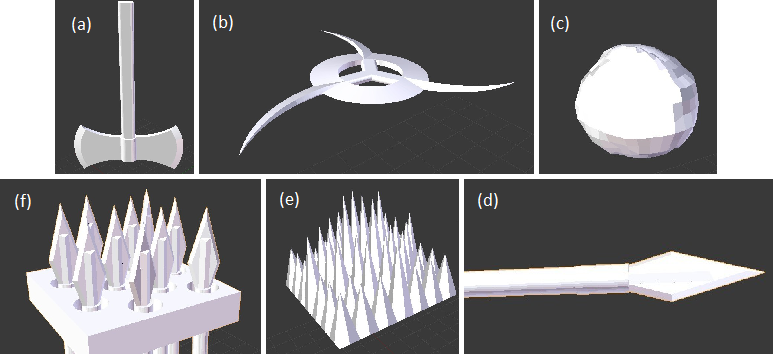
\includegraphics[width=\textwidth]{hazards}
\caption[Hazards found in the game.]{Hazards found in the game.  (a) Swinging Axe.  (b) Saw Blade.  (c) Boulder.  (d) Javelin.  (e) Spikes.  (f) Spear Trap.} \label{fig:hazards}
\end{center}
\end{figure}


\subsubsection{Score}
When a stage is completed you will receive a score expressed as a star-rating.  This rating ranges from 1 star to 3 stars and is based on the time taken to complete the stage.  Try to achieve a 3-star rating on every stage!


\subsection{Game Controls}
The default game controls are given in \hyperref[tab:ctrl]{Table~\ref*{tab:ctrl}}.  In the current version of the game, the controls cannot be remapped.


\begin{table}[H]
\caption{Game Controls} \label{tab:ctrl}
\centering
\begin{tabularx}{0.65\textwidth}{p{2.5cm}X}
\toprule {\bf Key} & {\bf Function}\\
\midrule
A & Move left\\
D & Move right\\
SPACE & Jump\\
ESC & Open menu (pauses game)\\
\bottomrule
\end{tabularx}
\end{table}

\section{Level Editor}
\label{sec:edit}
{\center ***************\\}
\noindent LEVEL EDITOR GUIDE TO BE COMPLETED AFTER LEVEL EDITOR IS COMPLETE!
{\center ***************\\}

\section{FAQ}
\label{sec:faq}
{\center ***************\\}
\noindent TO BE COMPLETED AFTER USER EXPERIENCE SURVEY.  CURRENTLY NO FREQUENTLY ASKED QUESTIONS...
{\center ***************\\}

\section{Troubleshooting}
\label{sec:trouble}
\subsection{Compilation Errors}
\subsubsection{\emph{\texttt{CMake} fails to generate build files.}}
\noindent Ensure that you have \texttt{\bf gcc} installed.  If this is not the issue, refer to the documentation provided at \href{http://www.cmake.org}{cmake.org} for further troubleshooting.

\subsubsection{\emph{The compilation process fails while running the makefile.}}
\noindent The makefile generated by \texttt{\bf CMake} provides detailed error reporting.  In most cases failure results from a missing function or library.  Instructions for resolving a particular issue can usually be found via an online search of the error message.

\subsubsection{\emph{\texttt{CMake} is using an older/wrong version of \texttt{\bf gcc} or defaulting to a different compiler.}}
\noindent If you are using Windows, ensure that the desired version of \texttt{\bf gcc} appears before all others in your PATH variable.  If a different compiler is being used by \texttt{\bf CMake}, double check that you are inputting the correct command (the \texttt{MinGW Makefiles} generator should default to \texttt{\bf gcc}).\\

\noindent If you are using OS X or Linux, you can explicitly select the compiler by exporting the CC and CXX environment variable prior to calling \texttt{\bf CMake} using the following commands:\\

\noindent \qquad \texttt{export CC = path\char`_to\char`_gcc}\\
${}$\noindent \qquad \texttt{export CXX = path\char`_to\char`_g++}


\subsubsection{\emph{I am trying to use a compiler that is not \texttt{gcc} with the installer and it is not working.}}
\noindent \texttt{\bf gcc} is the only officially supported compiler at this time.  Other compilers may or may not work with the provided installer and their use is not advised.  If you are determined to use a different compiler, manual installation is recommended.  Modifications to the source code of the game and/or the libraries may be required.


\subsection{Runtime Errors}
\subsubsection{\emph{The game creates a terminal/command prompt window which immediately closes.}}
\noindent This indicates that the game has encountered a startup error.  Try running the game from the terminal/command prompt so that any error messages produced before the game exits remain visible.

\subsubsection{\emph{The game encounters an error while loading an object.}}
\noindent Check that the data folder in the \texttt{source} directory was copied into the \texttt{game} directory.

\subsubsection{\emph{The game encounters an error while loading a texture.}}
\noindent Check that the data folder in the \texttt{source} directory was copied into the \texttt{game} directory.

\subsubsection{\emph{The game encounters an error while loading a sound file.}}
\noindent Check that the data folder in the \texttt{source} directory was copied into the \texttt{game} directory.

\subsubsection{\emph{The game encounters an error while loading shaders and complains about an unsupported GLSL version.}}
\noindent GLSL v330 is required to run the game.  This message indicates that your system does not support OpenGL v3.3.

\subsubsection{\emph{I am using a system with a GPU that supports OpenGL v3.3 or higher but the game does not run.}}
\noindent Make sure that your GPU drivers are up to date.

\subsubsection{\emph{I am using a notebook that supports OpenGL v3.3 or higher but the game does not run.}}
\noindent This can happen if you are using a notebook computer with both an integrated and a dedicated GPU.  Your notebook may be using the integrated GPU by default, in which case you will need to explicitly tell your system to run the game executable with the dedicated GPU.  Instructions for doing this vary and are beyond the scope of this guide.


\subsection{General Troubleshooting}
{\center ***************\\}
\noindent THIS SECTION WILL COVER ANY IN-GAME ISSUES THAT MAY OCCUR.  TO BE COMPLETED AFTER USER EXPERIENCE SURVEY.
{\center ***************\\}


\end{document}
